\documentclass[a4paper, 12pt]{report}
\usepackage{graphicx}
\usepackage{xspace}
\usepackage[margin= 1in,includefoot]{geometry}
\newcommand\nth{\textsuperscript{th}\xspace}
\usepackage{xcolor}
\usepackage{lipsum}
\usepackage{listings}
\begin{document}
\begin{figure}
\includegraphics[scale=.63]{medipol.png}
\centering
\end{figure}
\begin{titlepage}
\title{Fall 2021, Computer Vision \\ Homework 3}
\author{by 64160010 - Rumeysa ÇELİK}
\maketitle
\end{titlepage}
\section*{{\textbf{Problem Set 3}}}
\textbf{Problem 1:}
\begin{itemize}
\item[a.] Keypoints found first:
\begin{figure}[h]
\includegraphics[scale=.53]{1.png}
\centering
\caption{Image 1 Keypoints}
\end{figure}
\begin{figure}[h]
\includegraphics[scale=.53]{2.png}
\centering
\caption{Image 2 Keypoints}
\end{figure}
\newpage
\item[b.] answer:
\begin{figure}
\includegraphics[scale=.43]{3.png}
\centering
\caption{Matches}
\end{figure}
\begin{figure}[h]
\includegraphics[scale=.53]{4.png}
\centering
\end{figure}
\item[c.] answer:
\begin{figure}[h]
\includegraphics[scale=.53]{5.png}
\centering
\end{figure}
\newpage
\item[d.] answer:
\begin{figure}[h]
\includegraphics[scale=.43]{6.png}
\centering
\caption{Residual Image}
\end{figure}
\item[e.] answer:
\begin{figure}[h]
\includegraphics[scale=.43]{7.png}
\centering
\caption{Stitched Image}
\end{figure}
\end{itemize}
\newpage
\setlength{\parindent}{0pt}{\textbf{Problem 2:}
\begin{itemize}
\item[a.] answers:
\begin{figure}[h]
\includegraphics[scale=.47]{8.png}
\centering
\caption{Optical Flow Horizontal
and Optical Flow Vertica}
\end{figure}
\begin{figure}[h]
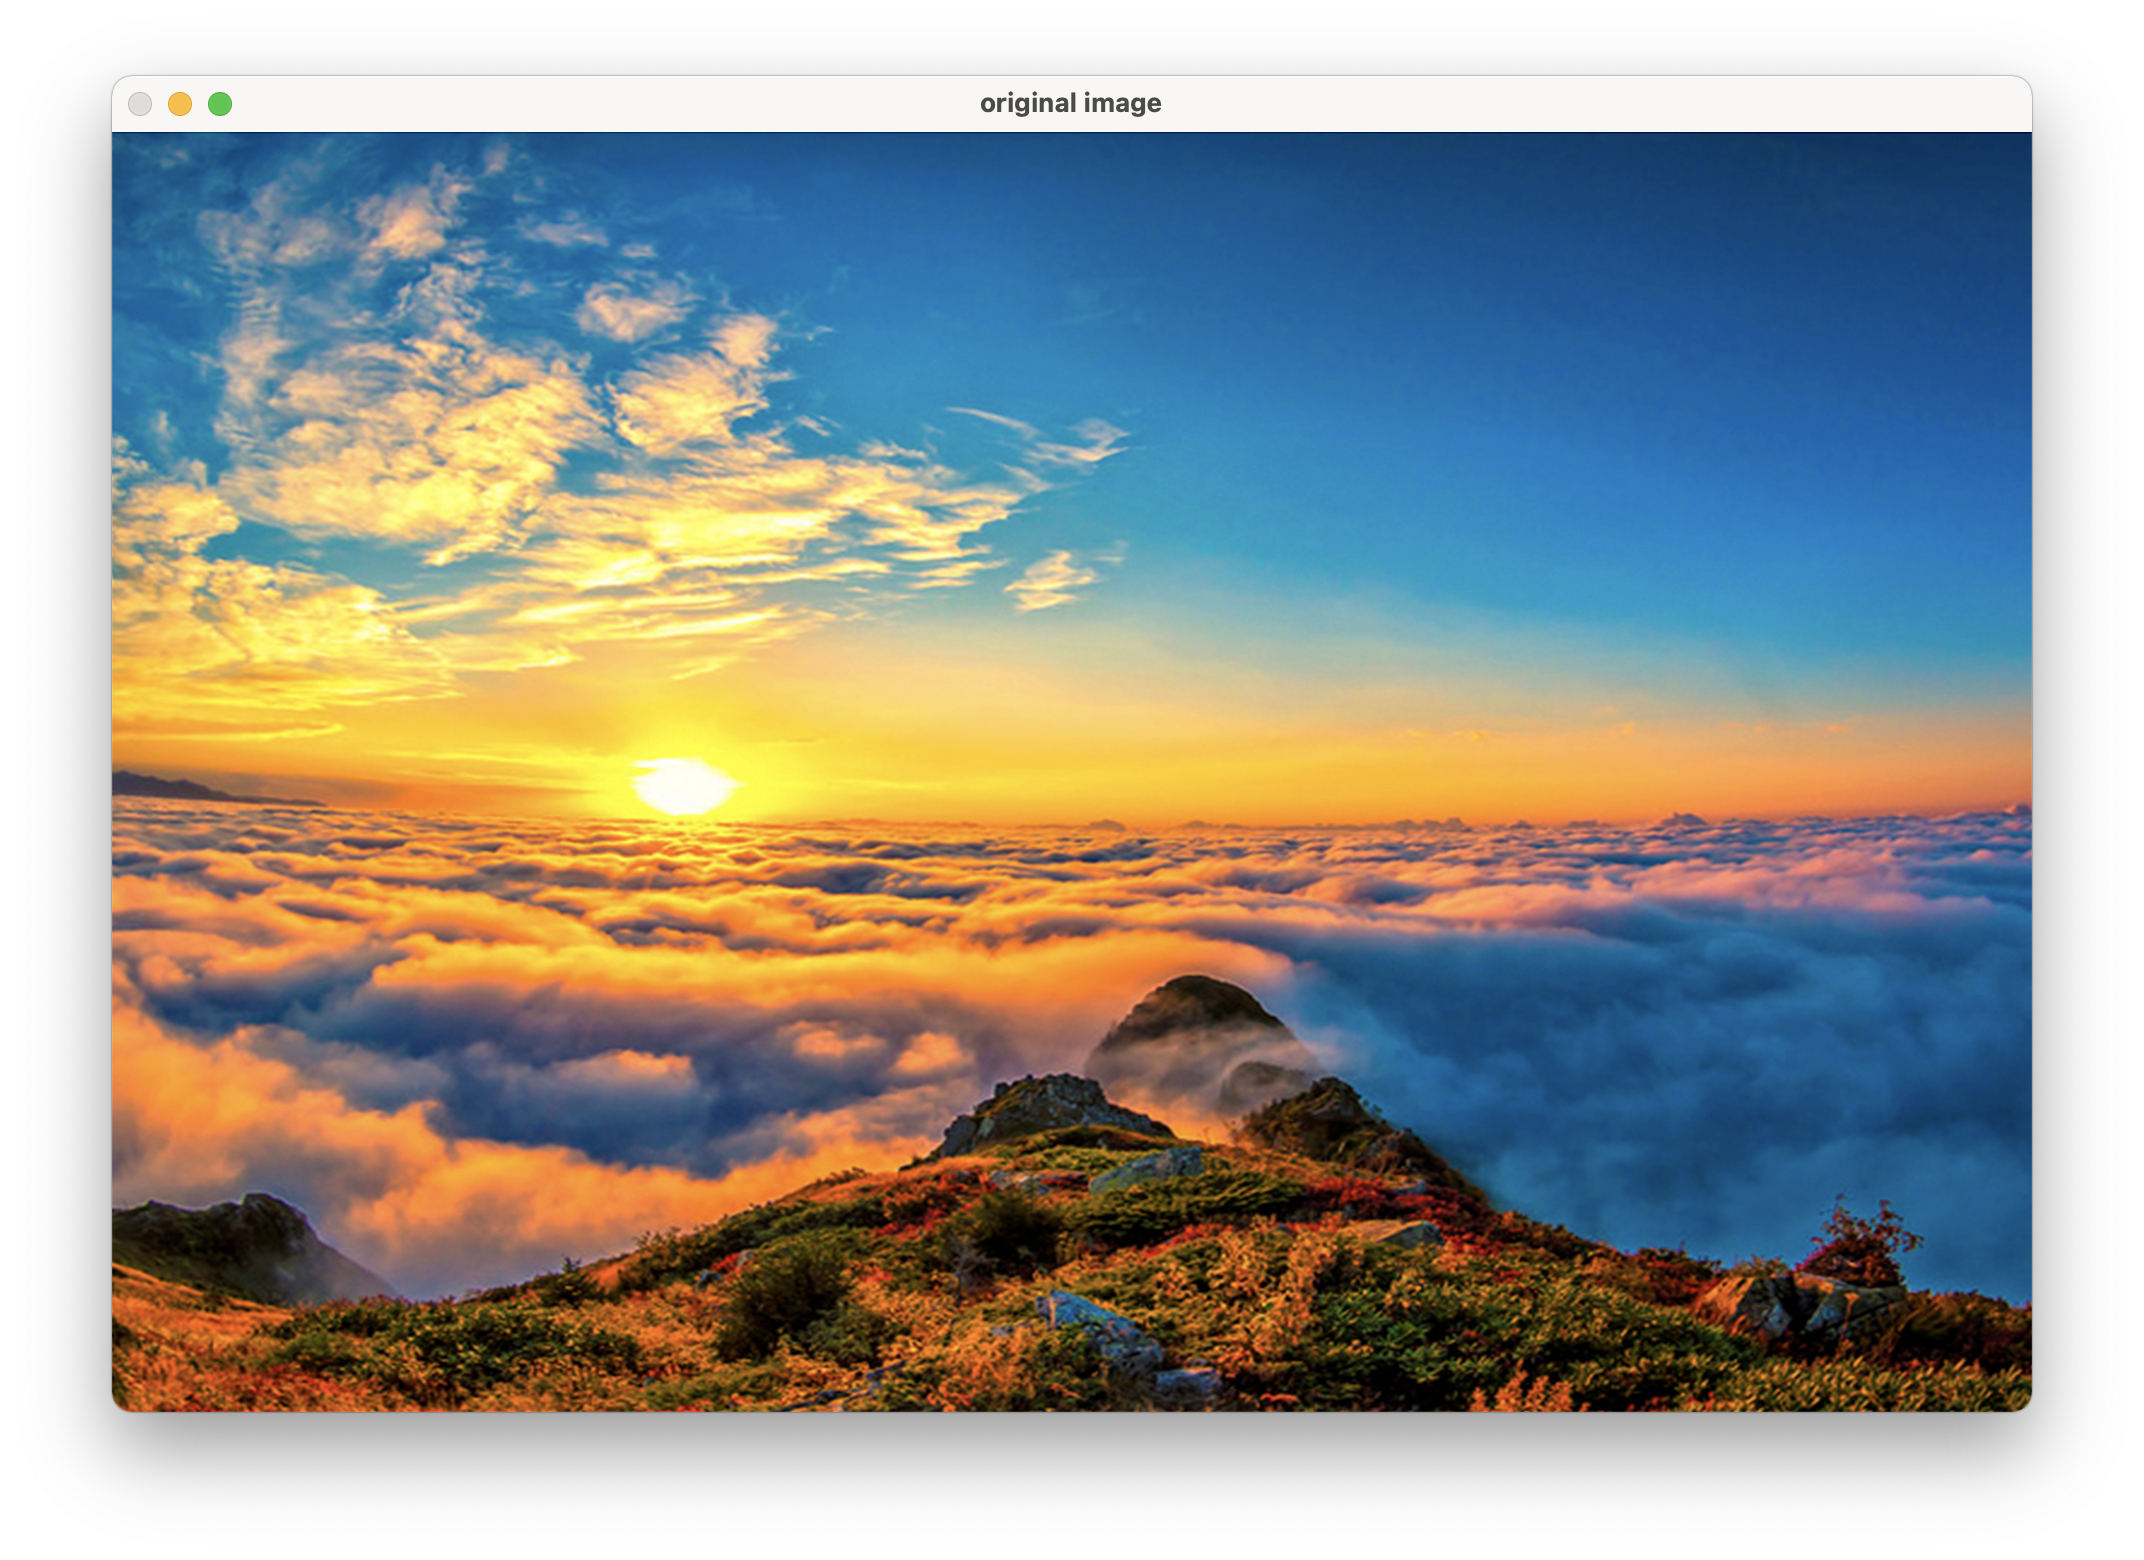
\includegraphics[scale=.47]{9.png}
\centering
\caption{Optical Flow Warped Image
and Optical Flow Residual}
\end{figure}
\newpage
\item[b.] answers:
\begin{figure}[h]
\includegraphics[scale=.43]{10.png}
\centering
\caption{Shi-Tomasi Corner Points Image 1
and Shi-Tomasi Corner Points Image 2}
\end{figure}
\begin{figure}[h]
\includegraphics[scale=.37]{11.png}
\centering
\caption{Tracking with Lucas Canade method}
\end{figure}
\end{itemize}































\end{document}